\documentclass[]{article}
\usepackage[UTF8]{ctex}	% 中文语言包
\usepackage{multicol}  % 用于实现在同一页中实现不同的分栏
\usepackage{amsmath}	% 公式功能包
\usepackage[shortlabels]{enumitem}	% 编号扩展功能包

% 伪代码的格式设置
%%***************************************************************************************************
%% 头文件部分
%\makeatletter
%\newif\if@restonecol
%\makeatother
%\let\algorithm\relax
%\let\endalgorithm\relax
%\usepackage[linesnumbered,ruled,vlined]{algorithm2e}%[ruled,vlined]{
%\usepackage{algpseudocode}
%\renewcommand{\algorithmicrequire}{\textbf{Input:}}  % Use Input in the format of Algorithm
%\renewcommand{\algorithmicensure}{\textbf{Output:}} % Use Output in the format of Algorithm 
%%***************************************************************************************************



\usepackage{algorithm}
\usepackage{algorithmicx}
\usepackage{algpseudocode}

\floatname{algorithm}{算法}
\renewcommand{\algorithmicrequire}{\textbf{输入:}}
\renewcommand{\algorithmicensure}{\textbf{输出:}}



\usepackage{titlesec}  % 自定义多级标题格式的宏包

% \titleformat{command}[shape]  % 定义标题类型和标题样式,字体
% {format}  % 定义标题格式:字号(大小),加粗,斜体 例如 \fontsize{20.75pt}\bfseries\centering
% {label}  % 定义标题的标签,即标题的标号等
% {sep}  % 定义标题和标号之间的水平距离
% {before-code}  % 定义标题前的内容

\titleformat{\section}[block]%定义标题类型和标题样式,字体
{\Large\bfseries}  % 定义标题格式:字号(大小),加粗(,斜体),居中
{\bfseries\arabic{section}}  % 定义标题的标签,即标题的标号等
{0.5em}  % 定义标题和标号之间的水平距离
{}  % 定义标题前的内容
[]  % 定义标题后的内容

\titleformat{\subsection}[block]  % 定义标题类型和标题样式,字体
{\large\bfseries}  % 定义标题格式:字号(大小),加粗,斜体
{\bfseries\arabic{section}.\bfseries\arabic{subsection}}  % 定义标题的标签,即标题的标号等
{0.5em}  % 定义标题和标号之间的水平距离
{}  % 定义标题前的内容
[]  % 定义标题后的内容

\titleformat{\subsubsection}[block]  % 定义标题类型和标题样式,字体
{\normalsize\bfseries}  % 定义标题格式:字号(大小),加粗,斜体
{\bfseries\arabic{section}.\bfseries\arabic{subsection}.\bfseries\arabic{subsubsection}}  % 定义标题的标签,即标题的标号等
{0.5em}  % 定义标题和标号之间的水平距离
{}  % 定义标题前的内容
[]  % 定义标题后的内容

\titleformat{\paragraph}[block]
{\small\bfseries}
{[\arabic{paragraph}]}
{1em}
{}
[] 

% \titleformat{\section}[block]{\LARGE\bfseries}{\Roman{section}}{1em}{Hello: }[]
% \titleformat{\subsection}[block]{\Large\itshape\mdseries}{\arabic{section}.\arabic{subsection}}{0.5em}{}[]
% \titleformat{\subsubsection}[block]{\normalsize\bfseries}{\arabic{subsection}-\arabic{subsubsection}}{0em}{}[]
% \titleformat{\paragraph}[block]{\small\bfseries}{[\arabic{paragraph}]}{1em}{}[]



\usepackage{setspace}  % 设置行间距
\usepackage{geometry}  % 设置一些页面格式,还没开发安全
\geometry{a4paper,left=2.0cm,right=2.0cm,top=2.25cm,bottom=2.0cm}

% 正文字体的设置
\PassOptionsToPackage{no-math}{fontspec}
\usepackage{mathspec}
\setmainfont{Times New Roman}  % 正文英文字体的设置
\setCJKmainfont{SimSun}[AutoFakeBold,ItalicFont=KaiTi]  % 正文中文字体的设置
\setCJKsansfont{SimHei}%对应sf无衬线
\setCJKmonofont{FangSong}%对应tt打字机
%\newCJKfontfamily{\kaishu}[AutoFakeBold={2.17}]{STXingkai}


% 摘要格式的设置
\usepackage{tikz}
\usetikzlibrary{shapes,shadows}
\tikzstyle{abstractbox} = [draw=black, fill=white, rectangle, 
inner sep=20pt, style=rounded corners, drop shadow={fill=black,
	opacity=0.5}]
\tikzstyle{abstracttitle} =[fill=white]

\newcommand{\boxabstract}[2][fill=white]{
	\begin{center}
		\begin{tikzpicture}
			\node [abstractbox, #1] (box)
			{\begin{minipage}{0.82\linewidth}
					\setlength{\parindent}{2mm}
					\small #2
			\end{minipage}};
			\node[abstracttitle, right=10pt] at (box.north west) {\textbf{摘要}};
		\end{tikzpicture}
	\end{center}
}
	
	
%\newsavebox{\myabstractbox}
%\providecommand{\abstractnode}[2]{
	%	\begin{tikzpicture}%
		%		\node [abstractbox, fill=#1](box)%
		%		{#2};%
		%		\node[abstracttitle, right=10pt] at (box.north west) {Abstract};
		%	\end{tikzpicture}
	%}
%
%
%\newenvironment{abstractbox][1][white]{
%		\begin{center}%
	%			\def\abs@bgcok{#1}%
	%			\begin{Irbox}{\myabstractbox}
		%				\begin{minipage}{.80\linewidth}%% lparindent2em%
			%					\footnotesize #2
			%				\end{minipage}
		%			\end{Irbox}
	%%			\abstractnode{\abs@bgcol}{\usebox{\myabstractbox}}%
	%		\end{center}%
%	}
		
\makeatletter
\newenvironment{tablehere}
{\def\@captype{table}}
{}

\newenvironment{figurehere}
{\def\@captype{figure}}
{}
\makeatother
		


%opening
\title{图像语义切割(Image Semantic Segmentation)综述}
\author{{\small 计算机工程与技术学院 \quad\quad 周方全 | 202121081229 \quad\quad \textbf{邮件地址}:2542154447@qq.com}}
\date{}



\begin{document}
\maketitle  % 生成标题

%\begin{abstractbox}
%	{\bf 语义切割(Semantic Segmentation)是计算机视觉中十分重要的领域,它是指像素级别的识别图像,即
%		标注出每个像素所属的对象类别。此项技术目前广泛应用于医学图像与无人驾驶等领域。本文主要从语
%		义切割的基本概念介绍在深度学习引入前后此领域的算法发明与改进,侧重点在深度算法,从原始算法
%		全卷积网络(FCN)为切入点,引入一些其改进算法包括:Encoder-Decoder结构的U-net,具有更大感受野
%		的空洞卷积(Dilated Convolution)以及加入条件随机场(CRF)。 \rm} \newline	\newline	
%	{\bf\emph{ Key words-\ 语义切割; 归一化割; 全卷积网络; 空洞卷积; }\rm}	% 文字直接在创建好的环境中输入就可以了。编译后就可以看到效果。
%\end{abstractbox}
\boxabstract{	
	{   语义切割(Semantic Segmentation)是计算机视觉中十分重要的领域,它是指像素级别的识别图像,即
		标注出每个像素所属的对象类别。此项技术目前广泛应用于医学图像与无人驾驶等领域。本文主要从语
		义切割的基本概念介绍在深度学习引入前后此领域的算法发明与改进,侧重点在深度算法,从原始算法
		全卷积网络(FCN)为切入点,引入一些其改进算法包括:Encoder-Decoder结构的U-net,具有更大感受野
		的空洞卷积(Dilated Convolution)以及加入条件随机场(CRF)。 \rm} \newline	\newline	
	{   Key words-\ 语义切割; 归一化割; 全卷积网络; 空洞卷积; \rm}
}

\section{归约}

我们把问题分成两类,可以在多项式时间中求出结果的和不可以在多项式时间中求出结果的。
假如我们知道了一个问题$X$可以在多项式时间内解决。那我们还能用问题$X$的算法来解决其他问题吗?

我们称用一种问题的算法去解决其他问题的扩展方式 叫做归约。下面我们给出归约的定义:如果对于问题$X$任意的一个实例都能用以下两步解决:
\begin{enumerate}[i.]
	\item 多项式次数的标准计算 加上,
	\item 多项式次数调用可以解决问题$Y$的黑箱。
\end{enumerate}
那么我们就称问题$X$可以在多项式时间内归约到问题$Y$。记为:$ X \leq_P Y $。

\begin{figure}[htbp]
	\centering
	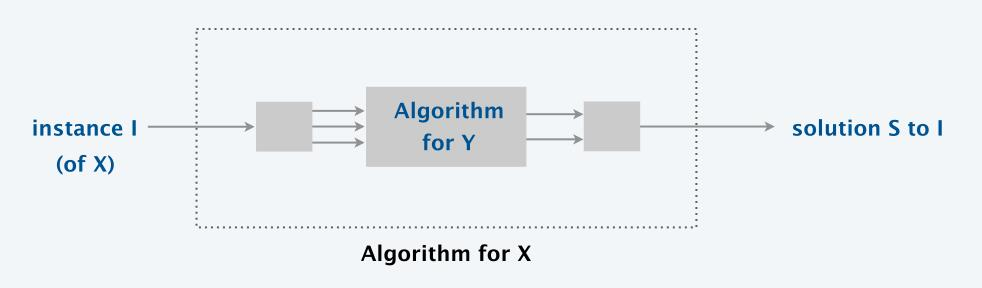
\includegraphics[width=1\linewidth]{picture/01}
	\caption{归约定义示意图}
	\label{fig:1}
\end{figure}
我们可以用图 \ref{fig:1} 任一给出一个问题$X$的一个实例我们花费多项式时间把它写入黑箱(姑且称为问题$Y$的算法,之所以成为黑箱,是因为问题$Y$可能也没有很好的已有算法),
所以问题$Y$的实力的大小一定是多项式的。那么问题$X$就可以得到解决。我们把这种归约称为 Cook 归约。显然归约具有递归性,即如果$ X \leq_P Y $并且$ Y \leq_P Z $ 那么,$ X \leq_P Z $。

我们定义归约,是为了把问题按照求解的难度进行分类。因为简单地问题可以归约到复杂的问题上去,而难的问题不可以归约到简单地问题上来。因为一个用来解决简单的问题的算法在碰到更加难的问题时就会行不通。

用归约设计算法。\textbf{如果$ X \leq_P Y $并且问题$Y$可以在多项式时间中得到解决,那么问题$X$也可以在多项式时间内得到解决。} 问题$X$ 可以归约到问题$Y$,那么本质上问题$X$不会比问题$Y$更加难,那么适用于问题$Y$的算法也一定在经过多项式时间处理后适用于问题$X$。

用归约来证明问题是不可解。\textbf{如果$ X \leq_P Y $并且问题$X$不可以在多项式时间中得到解决,那么问题$Y$也一定不可以在多项式时间内得到解决。}

用归约来证明两个问题多项式可解的等价性。如果$ X \leq_P Y $并且$ Y \leq_P X $, 那么我们会得到$ X \equiv_P Y $。只要这两个问题一个得到解决,那么另外一个问题就能得到解决。

对不同问题之间建立归约,往往需要很强的技巧性。3种常用的归约方法:
\begin{enumerate}[i.]
	\item 简单地问题等价性的归约
	\item 从特殊情形到一般情形的归约
	\item 使用小装置来完成归约
\end{enumerate}
后面在实例中我们会一一介绍。

简单地问题等价性的归约 的实例

证明:独立集问题$ \equiv_P $点覆盖问题

从特殊情形到一般情形的归约 的实例

证明:点覆盖问题 $ \leq_P $ 集合覆盖问题

使用小装置来完成归约 的实例

证明:3-SAT问题 $ \leq_P $ 独立集问题



\section{自身归约}

本质是把搜索问题规约为相应的判定问题。


\section{$\mathcal{NP}$}

\section{}
	
\begin{algorithm}[H]
	\caption{找到大小为$ K $的团}
	\KwIn{一张图$ G(V, E) $,团的大小$ k $}
	\KwOut{团大小为$ k $的顶点集合}
	\If{$ fun(G, k) \neq True $}
	{
		不存在这样的团\;	
		return None\;	
	}
	\For{ 顶点 $ v $ in $ V $ }
	{
		// 删除顶点 $ v $ 和其的相邻边\\
		$ V' = V - \{ v\} $\;
		$ E' = E - \{(u, v):u \in V\} $\;
		\If{$ fun(G, k) == True $}
		{
			$ V = V' $\;
			$ E = E' $\;
		}
		\If{$ \left| V \right| == k $}
		{
			break\;
		}
	}
	return V \;
\end{algorithm}

\section{$ \mathcal{NPC}$}

\section{}

\end{document}